\documentclass{standalone}
\usepackage[utf8]{inputenc}
\usepackage{tikz}
\usetikzlibrary{shapes.geometric, arrows}
\begin{document}

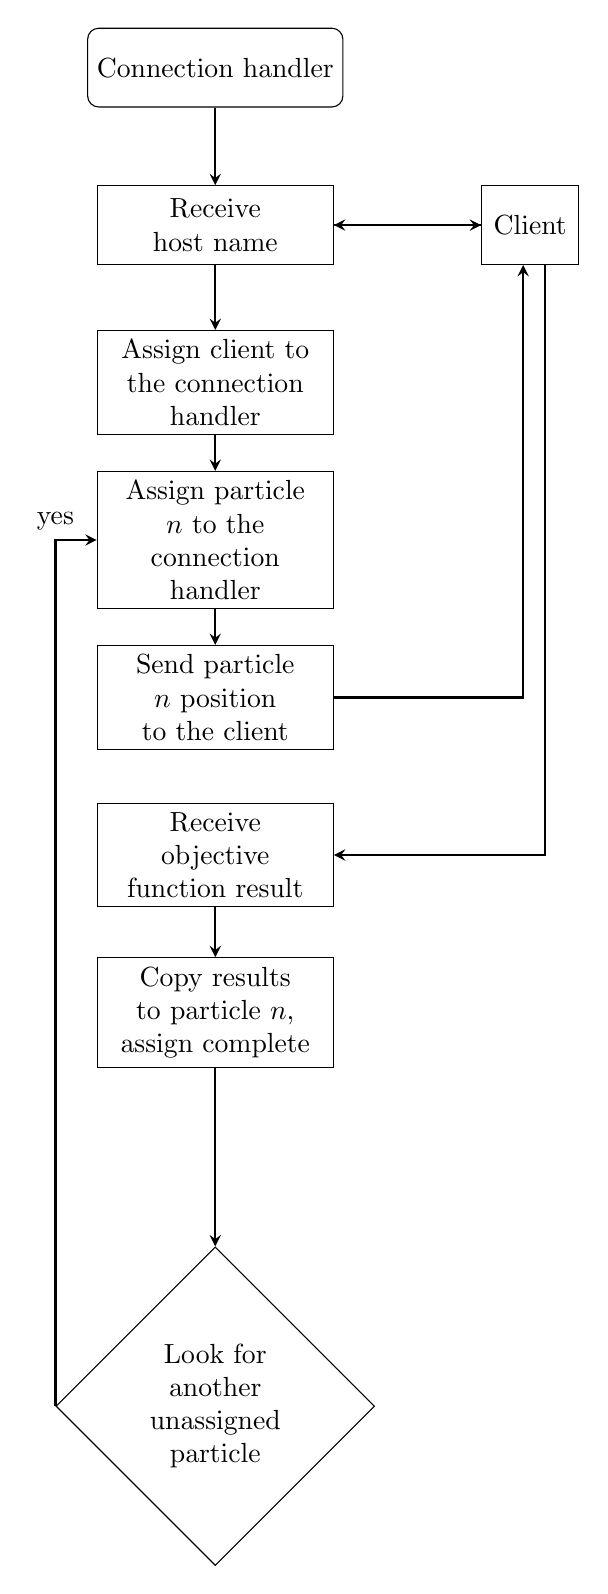
\begin{tikzpicture}[node distance=2cm]

\tikzstyle{program} = [rectangle, rounded corners, minimum width=3cm, minimum height=1cm,text centered, draw=black]
\tikzstyle{io} = [trapezium, trapezium left angle=70, trapezium right angle=110, minimum width=3cm, minimum height=1cm, text centered, draw=black]
\tikzstyle{process} = [rectangle, minimum width=3cm, minimum height=1cm, text centered, text width=2.5cm, draw=black]
\tikzstyle{comp} = [rectangle, minimum width=1cm, minimum height=1cm, text centered, text width=1cm, draw=black]
\tikzstyle{decision} = [diamond, minimum width=2.5cm, minimum height=0.5cm,text width =2cm, text centered, draw=black]
\tikzstyle{arrow} = [thick,->,>=stealth]


\node (conhandler) [program]                        {Connection handler};
\node (recv)       [process, below of = conhandler]      {Receive host name};
\node (assign)     [process, below of =recv]        {Assign client to the connection handler};
\node (client)     [comp, right of = recv, xshift=2cm]          {Client};
\node (particle)   [process, below of =assign]      {Assign particle $n$ to the connection handler};
\node (send)       [process, below of = particle]   {Send particle $n$ position to the client};
\node (recv2)      [process, below of = send]       {Receive objective function result};
\node (copy)       [process, below of = recv2]      {Copy results to particle $n$, assign complete};
\node (dec1)       [decision, below of = copy, yshift = -3cm]      {Look for another unassigned particle};

\draw [arrow] (conhandler) -- (recv);
\draw [arrow] (recv) -- (assign);
\draw [arrow] (recv) -- (client);
\draw [arrow] (client) -- (recv);
\draw [arrow] (assign) -- (particle);
\draw [arrow] (particle) -- (send);

\draw [arrow] (recv2) -- (copy);
\draw [arrow] (copy) -- (dec1);
\draw [arrow] (client.290) |- (recv2.east);
\draw [arrow] (send.east) -| (client.260);

\draw [arrow] (dec1.west) |- node[anchor=south] {yes} (particle.west);
\end{tikzpicture}

\end{document}

